\documentclass{article}

\usepackage{a4wide}
\usepackage[utf8]{inputenc}
\usepackage[T1]{fontenc}
\usepackage[french]{babel}
\usepackage[babel=true]{csquotes} % guillemets français
\usepackage{graphicx}
\graphicspath{{Images/}}
\usepackage{color}
\usepackage{hyperref}
\hypersetup{colorlinks,linkcolor=,urlcolor=blue}
\usepackage{amsmath}
\usepackage{amssymb}


\title{Rapport jeu de dame, Android, IOS}
\author{Billy Ronico, Said Ismael, L3 informatique}
\date{\today}

\begin{document}

\maketitle % pour écrire le titre


\section{Introduction}
\label{section:intro} % pour faire référence à la section ailleurs (\ref{...} voir plus bas)

Dans le cadre de la licence informatique, plus précisément pour le projet de développement 
mobile, nous avons choisi de réaliser \textbf{un jeu de dame} sur Android (Kotlin) et IOS (Swift).

\section{\textit{Regle du jeu de dame}~\cite{regleJeuDame}} 

\begin{itemize}
  \item Le jeu se joue à 2 joueurs sur un plateau de taille n * n.
  \item Les joueurs jouent chacun à leur tour. Les blancs commencent toujours.
  \item Le but du jeu est de capturer tous les pions adverses. 
  \item Si un joueur ne peut plus bouger, même s'il lui reste des pions, il perd la partie. 
  \item Chaque pion peut se déplacer d'une case vers l'avant en diagonale. 
  \item Un pion arrivant sur la dernière rangée et s'y arrêtant est promu en « dame ».
  \item La dame se déplace sur une même diagonale d'autant de cases qu'elle le désire, en avant et en arrière.
  \item Un pion peut en prendre un autre en sautant par dessus le pion adverse
   pour se rendre sur la case vide située derrière celui-ci. Le pion sauté est retiré du jeu.
  \item La prise est obligatoire.
  \item Lorsque plusieurs prises sont possibles, 
  il faut toujours prendre du côté du plus grand nombre de pièces.
  \item La dame doit prendre tout pion situé sur sa diagonale 
  (s'il y a une case libre derrière) et doit changer de direction à chaque 
  fois qu'une  nouvelle prise est possible. 
\end{itemize}

\section{Description générale de l'application}

Voici une capture du menu principal et d'une partie du jeu

\begin{center}
  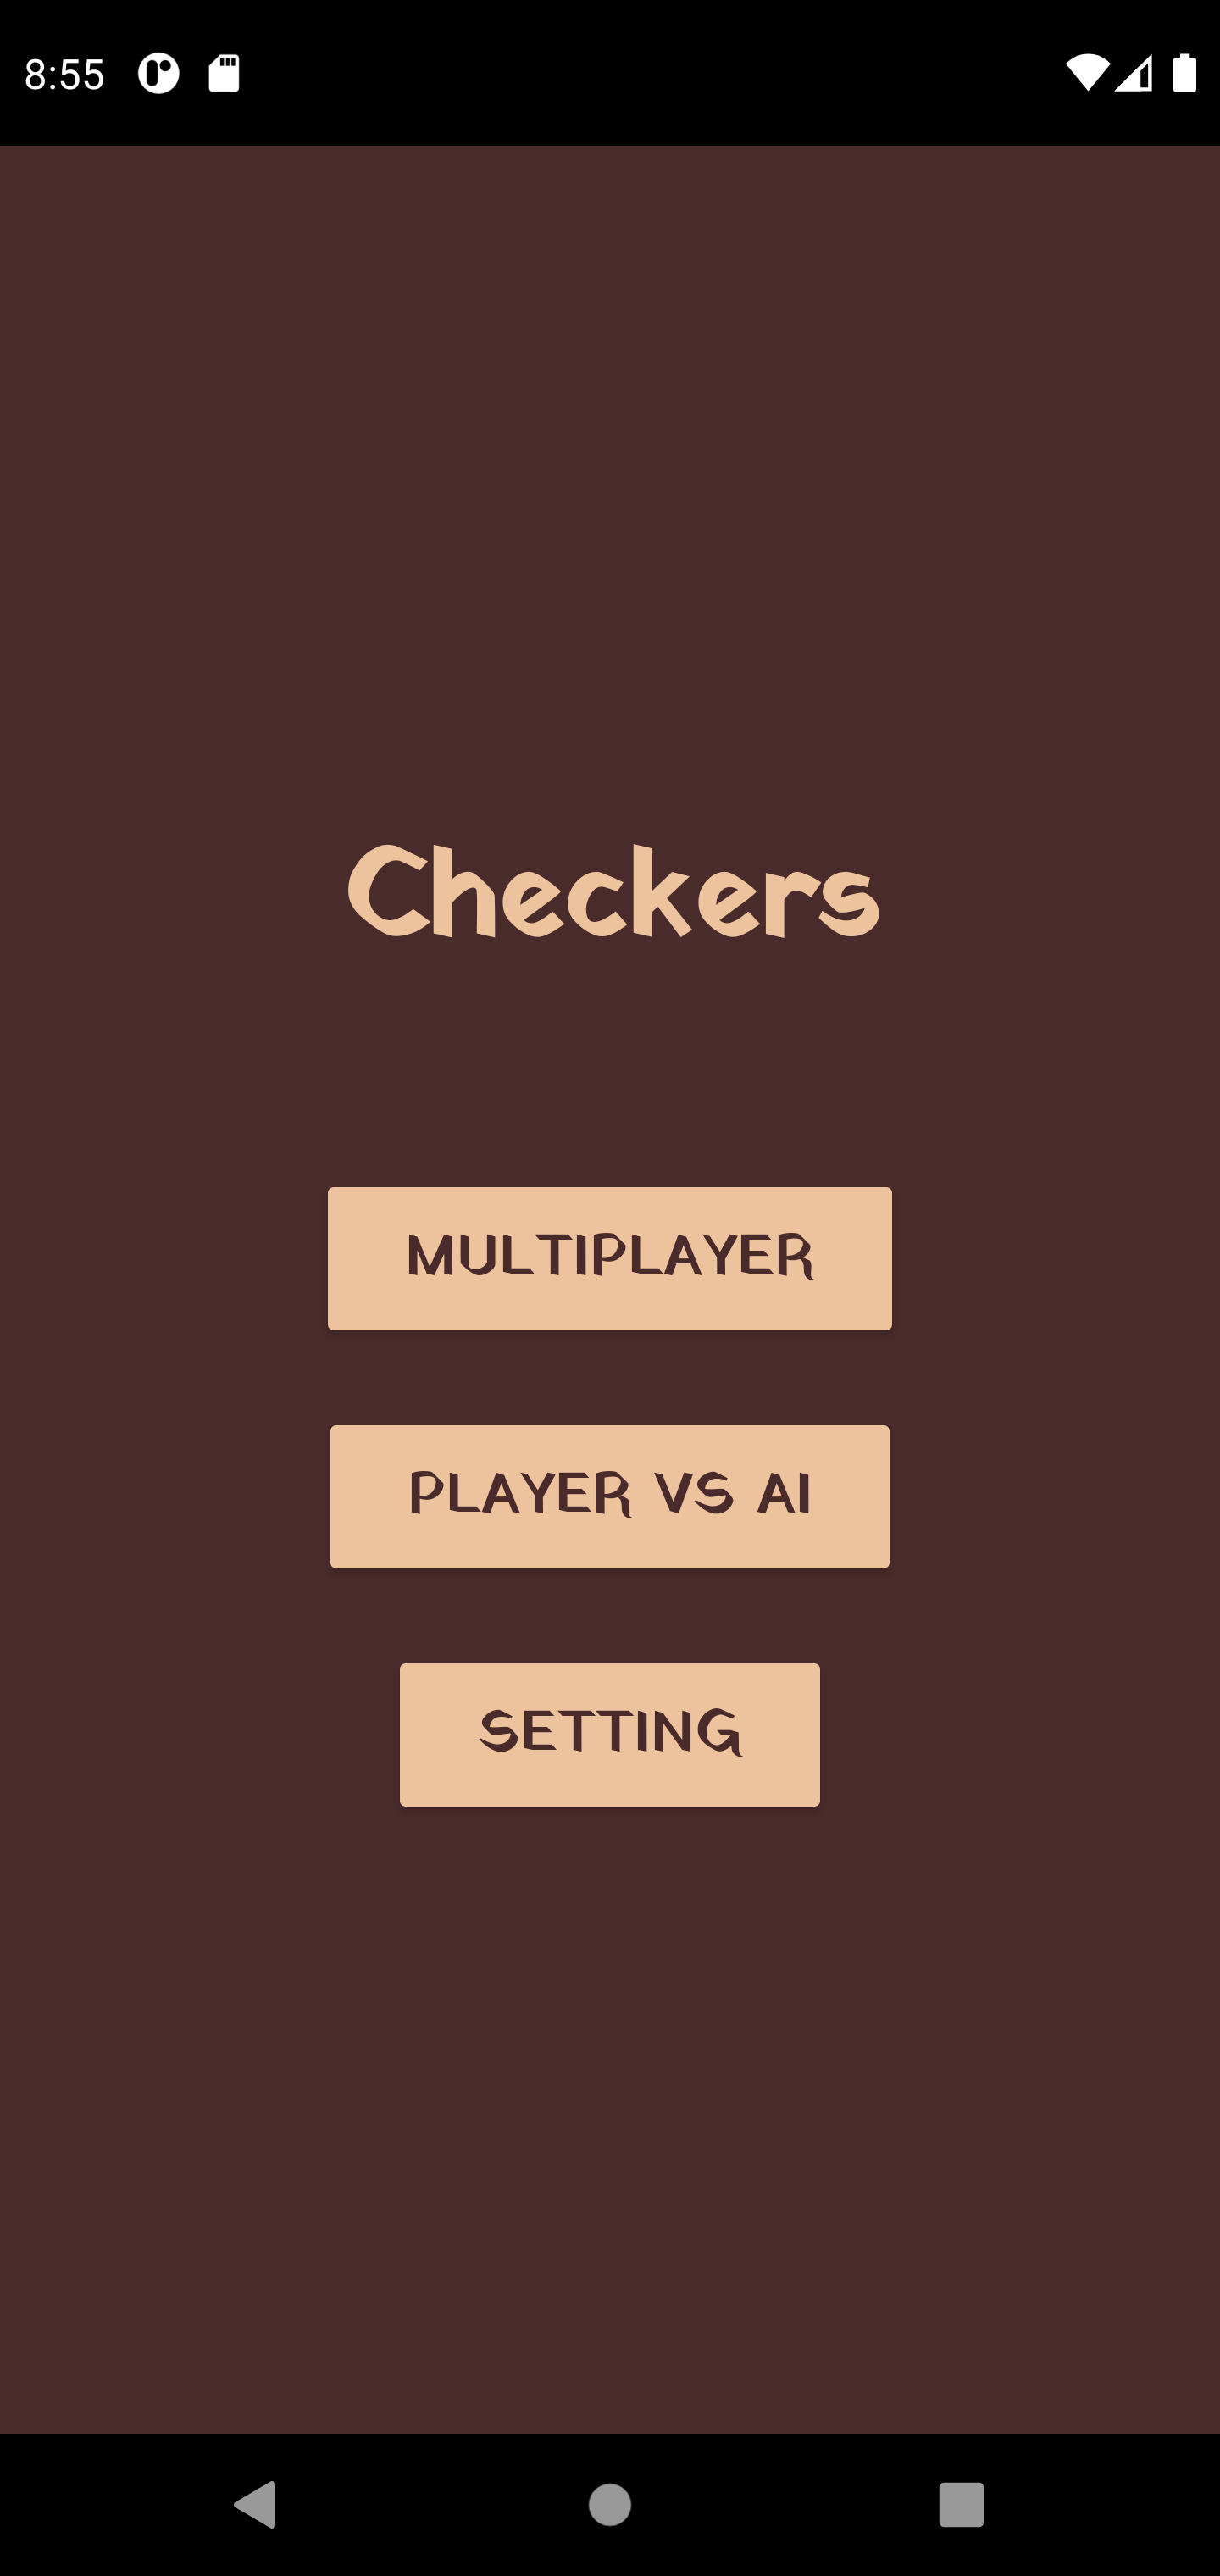
\includegraphics[scale=0.1]{menu_principal.png}
  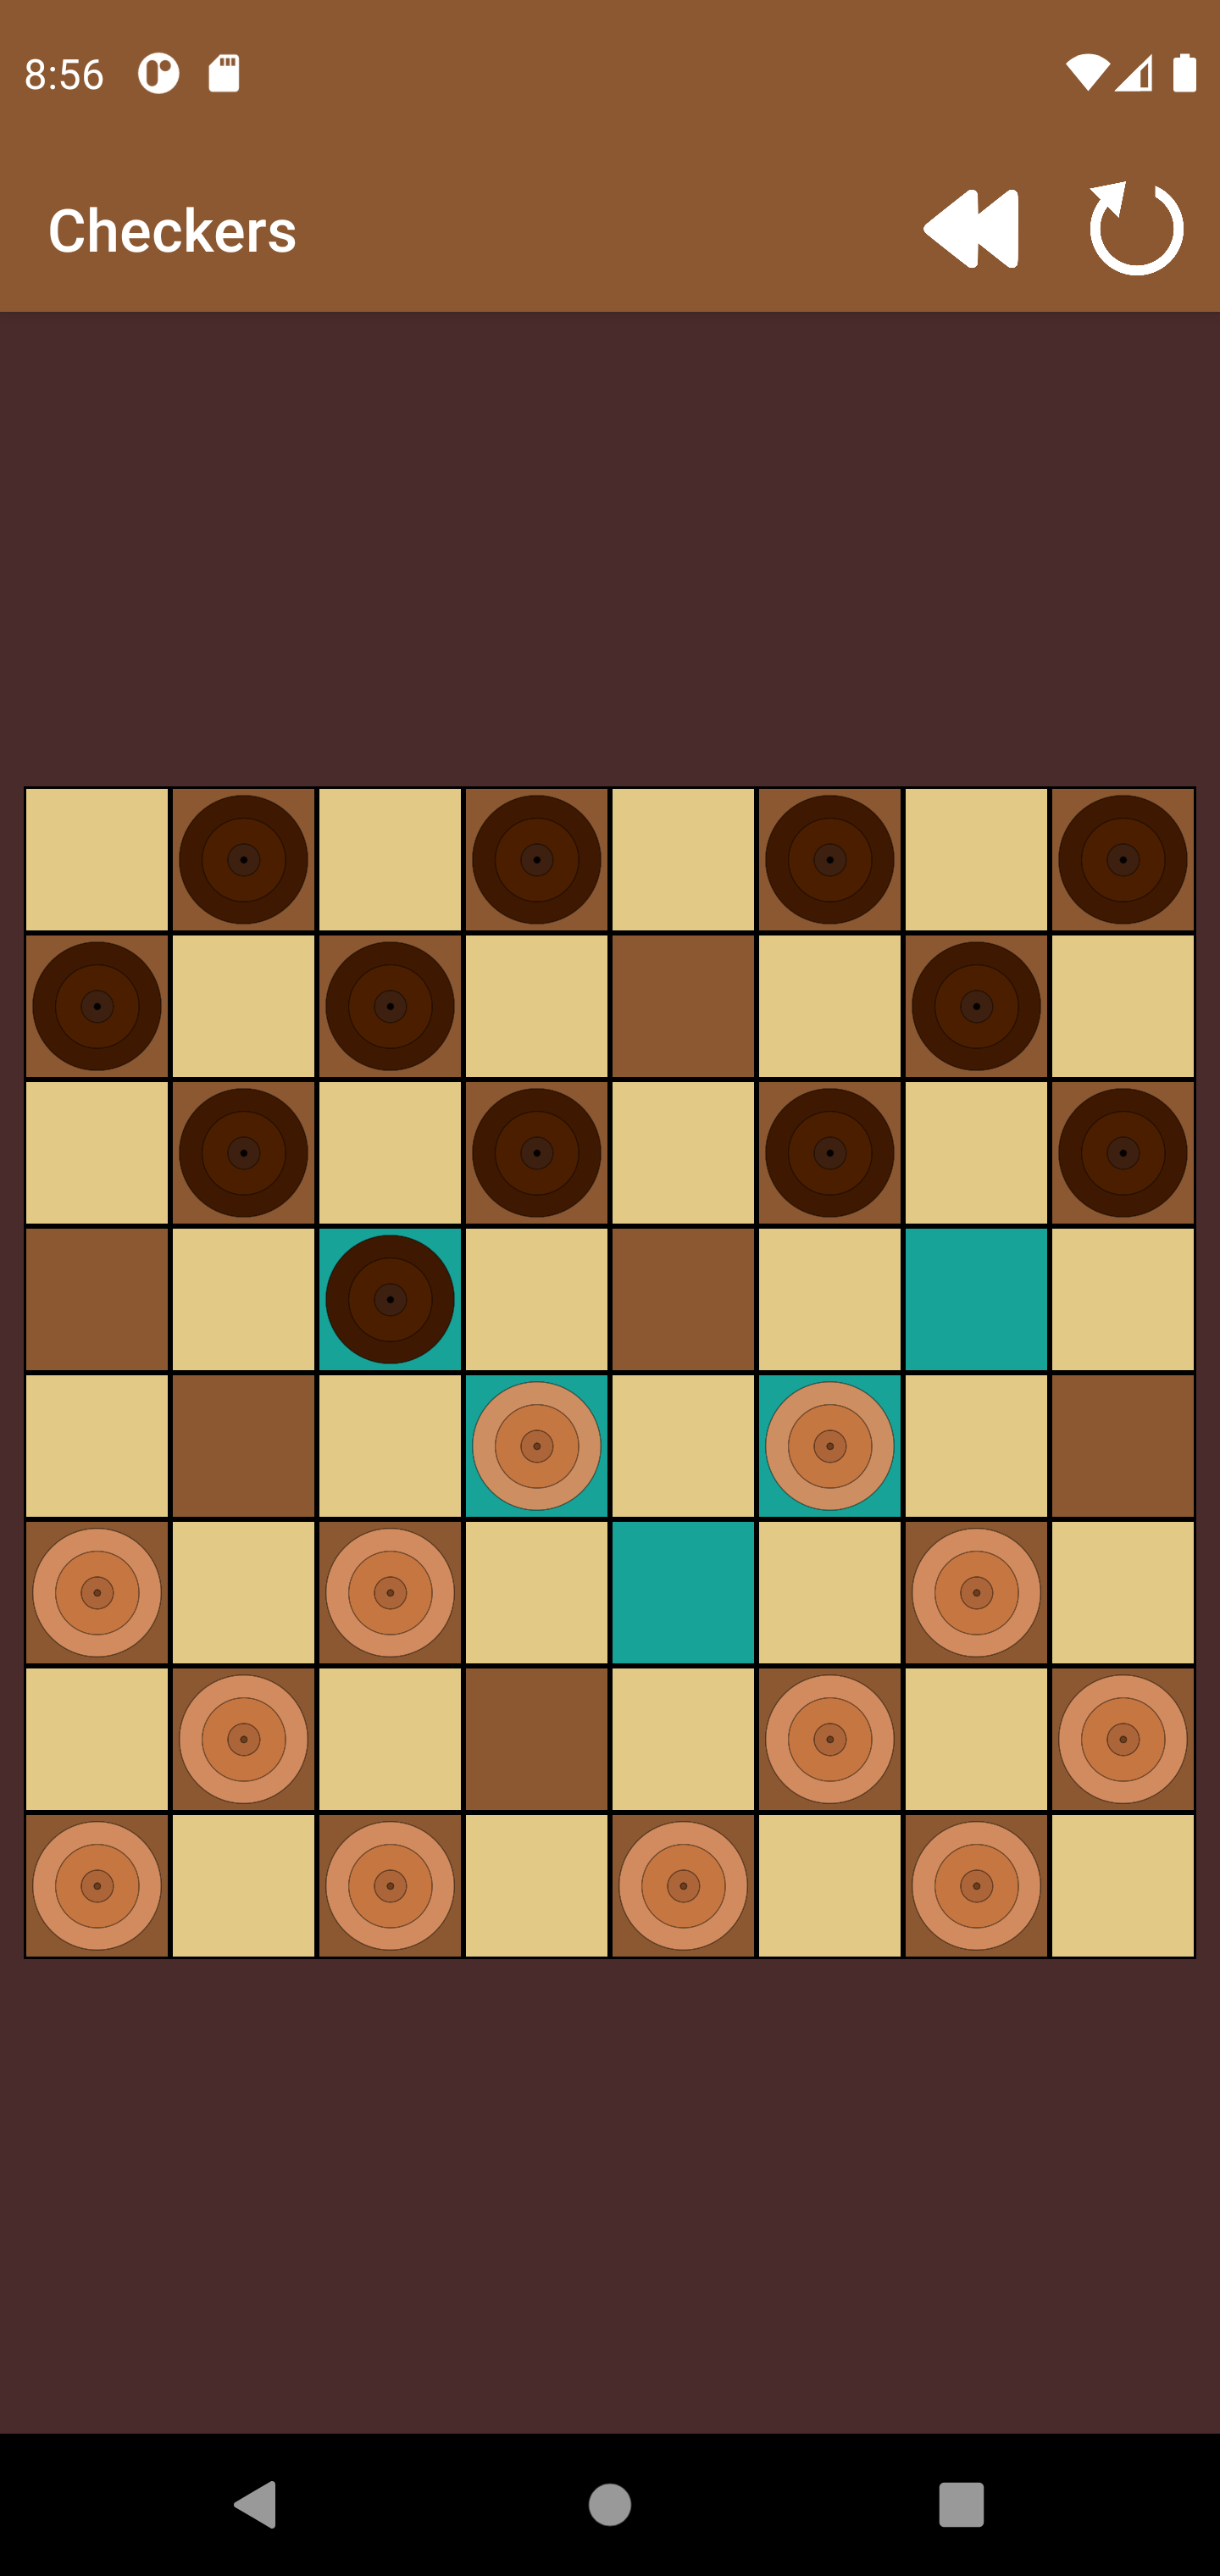
\includegraphics[scale=0.1]{partie_1.png}
\end{center}

\textbf{Fonctionnalités proposé par le jeu:}

\subsection{Un mode multijoueur:}

Ce mode consiste à faire affronté deux joueurs sur un même plateau de jeu.

Les joueurs jouent tour par tour sur les deux cotés du téléphone. 
De ce fait, pour des raisons d'IHM, on a décidé d'exclure le mode \textit{paysage} du jeu

\subsection{Un mode joueur contre une Inteligence Artificielle}

Ce mode consiste à faire affronté un joueur contre un IA.
L'IA a été implémenté en utilisant l'algorithme \textit{minimax}~\cite{miniMax}

\subsection{Paramètres}
Permet de personnaliser la couleur des cases, la taille du damier (6*6, 8*8, 10*10) 
et la difficulté de l'IA (Facile, Moyen, Difficile)

Ces paramètres une fois définie sera stockés dans un fichier et sera persistant.

\begin{center}
  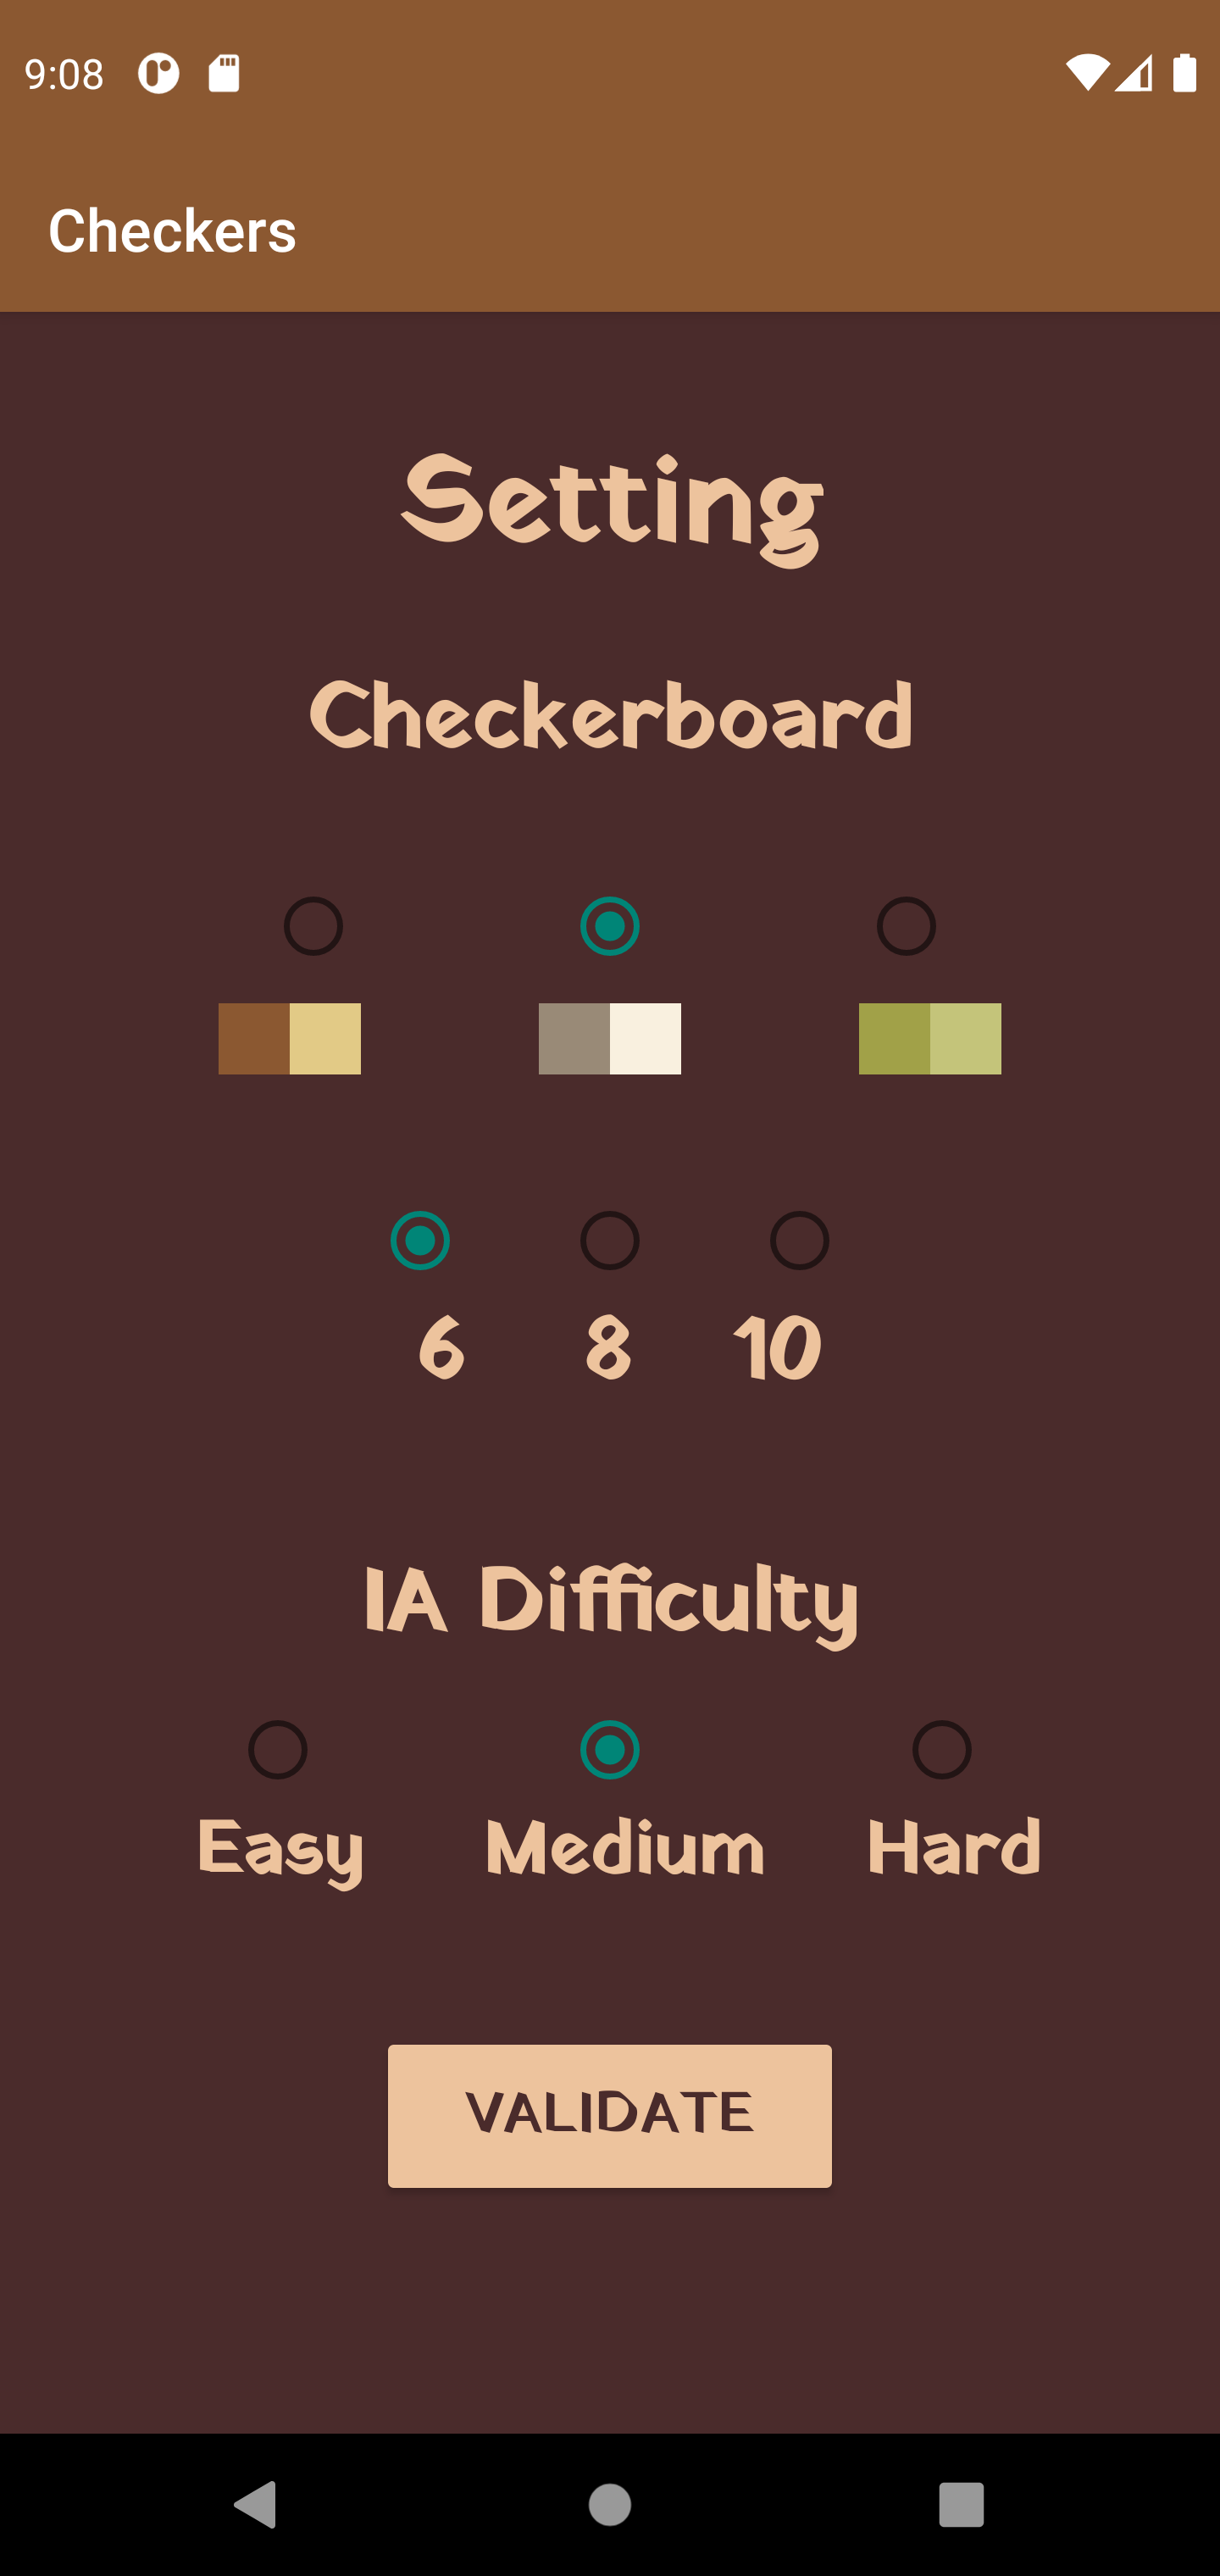
\includegraphics[scale=0.1]{setting_en.png}
  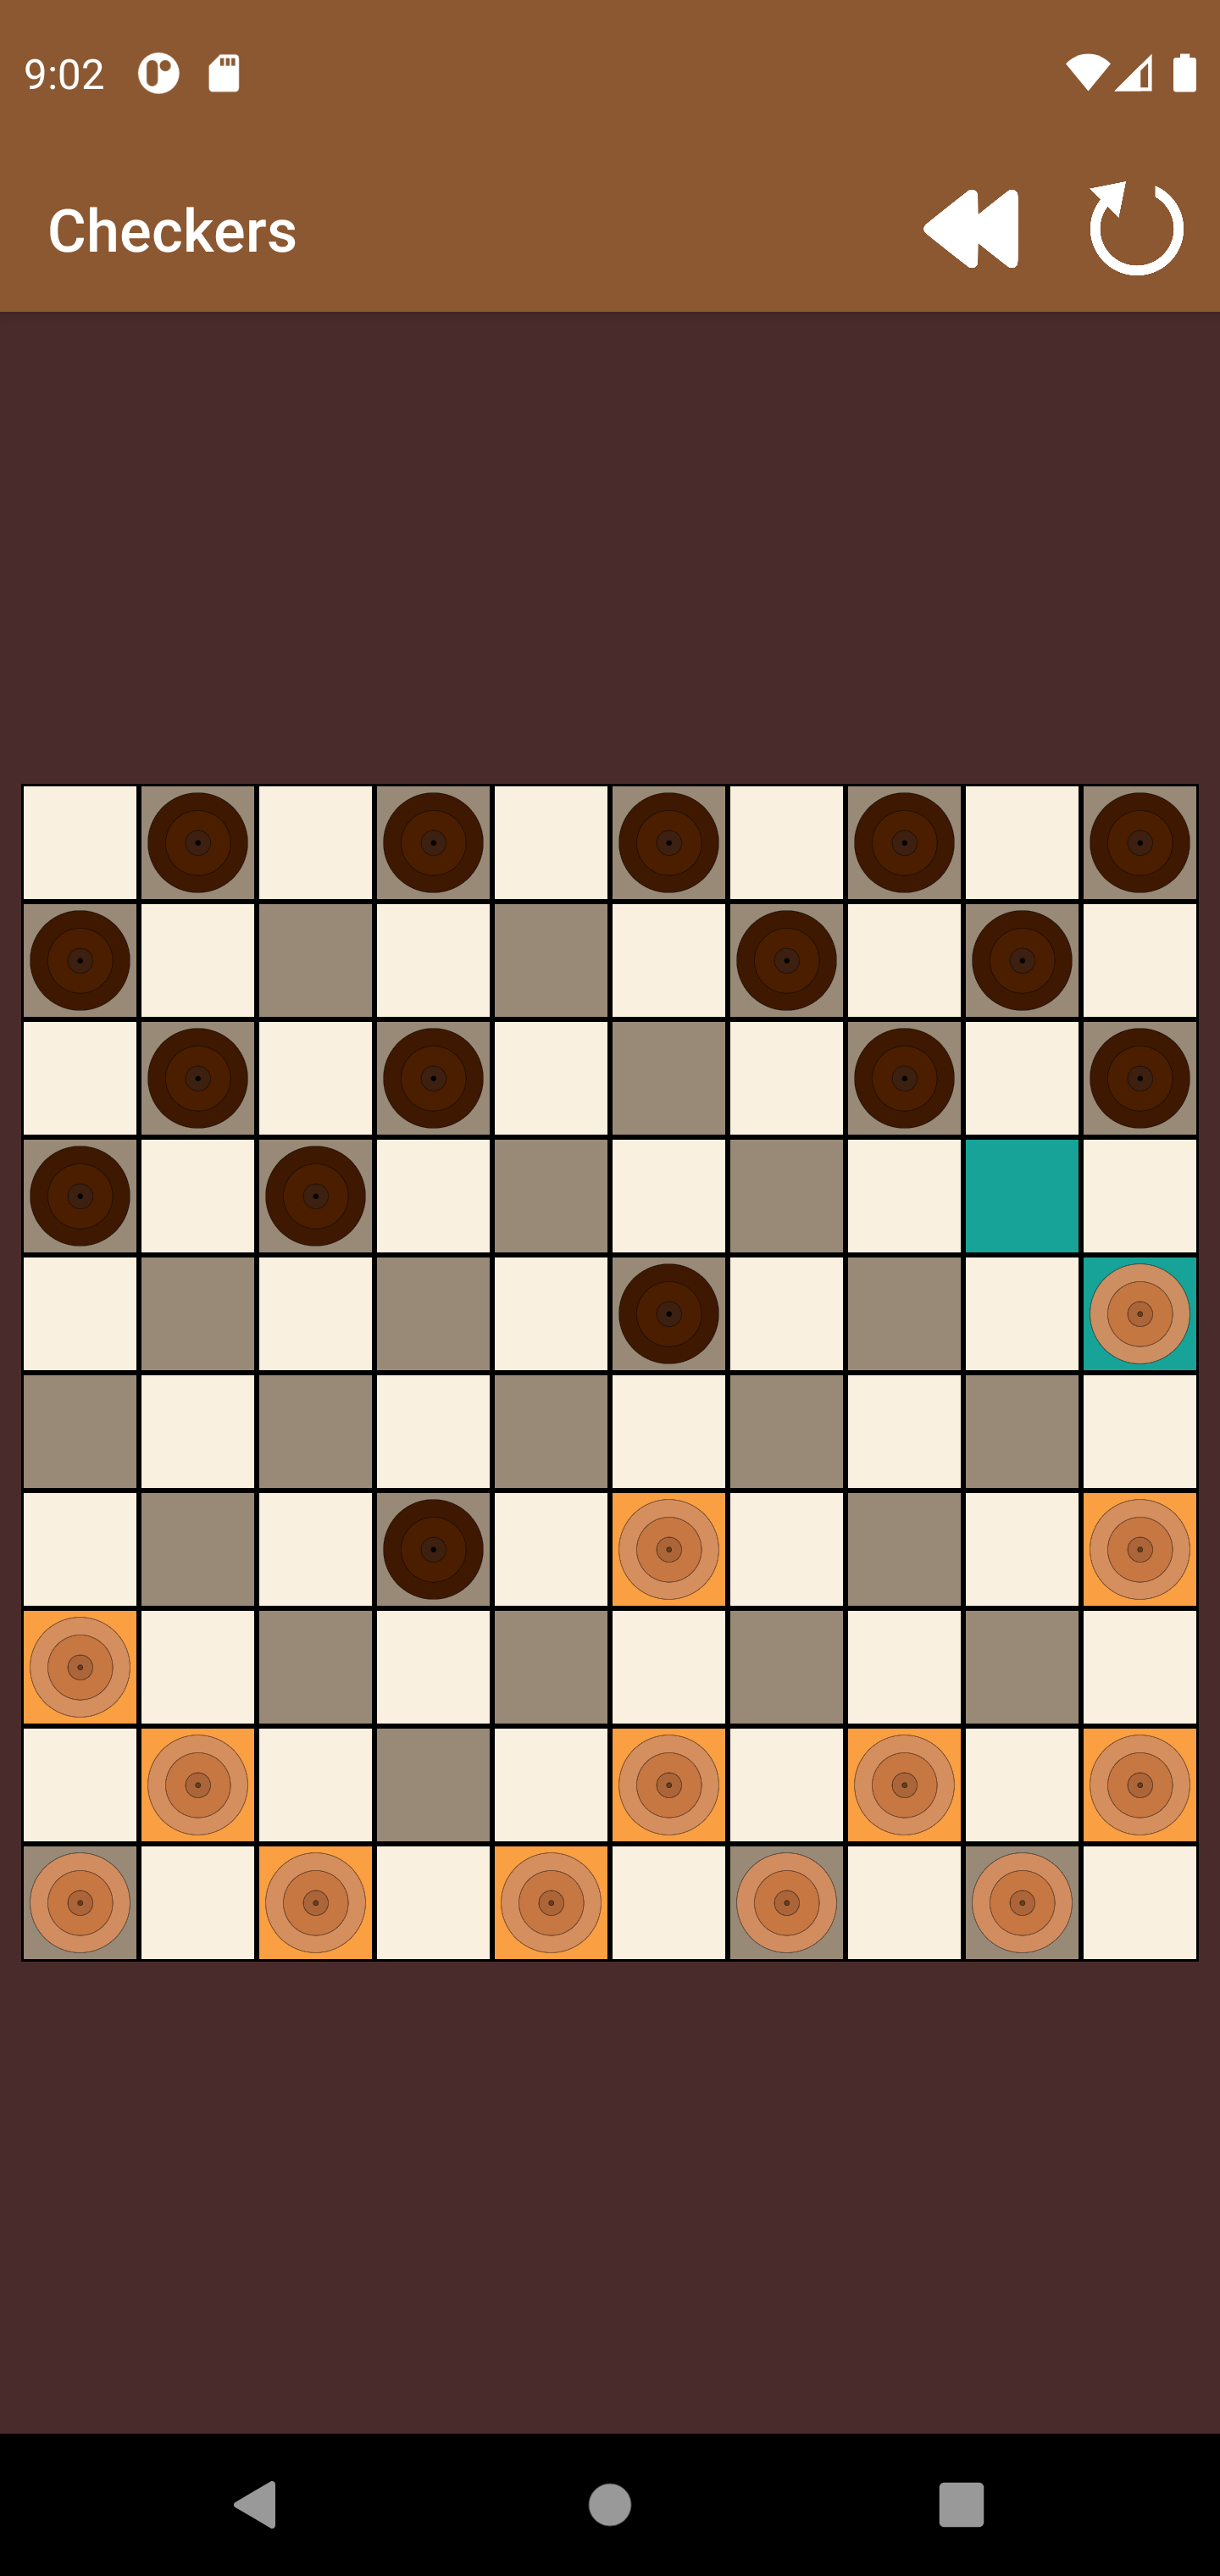
\includegraphics[scale=0.1]{partie_2.png}
\end{center}

\subsection{Option retour en arrière et Option restart Game}
Le bouton gauche de l'OptionMenu permet de revenir en arrière sur 
la partie en cours (disponible sur les 2 modes de jeu cité ci-dessus)

Le bouton droit de l'OptionMenu permet de rejouer la partie en cours.

\subsection{Application bilingue et responsive}

L'application est disponible en français (par défaut) et en anglais.

De plus, l'application est résponsive, c'est-à-dire qu'il s'adapte à toute les tailles d'écran

\begin{center}
  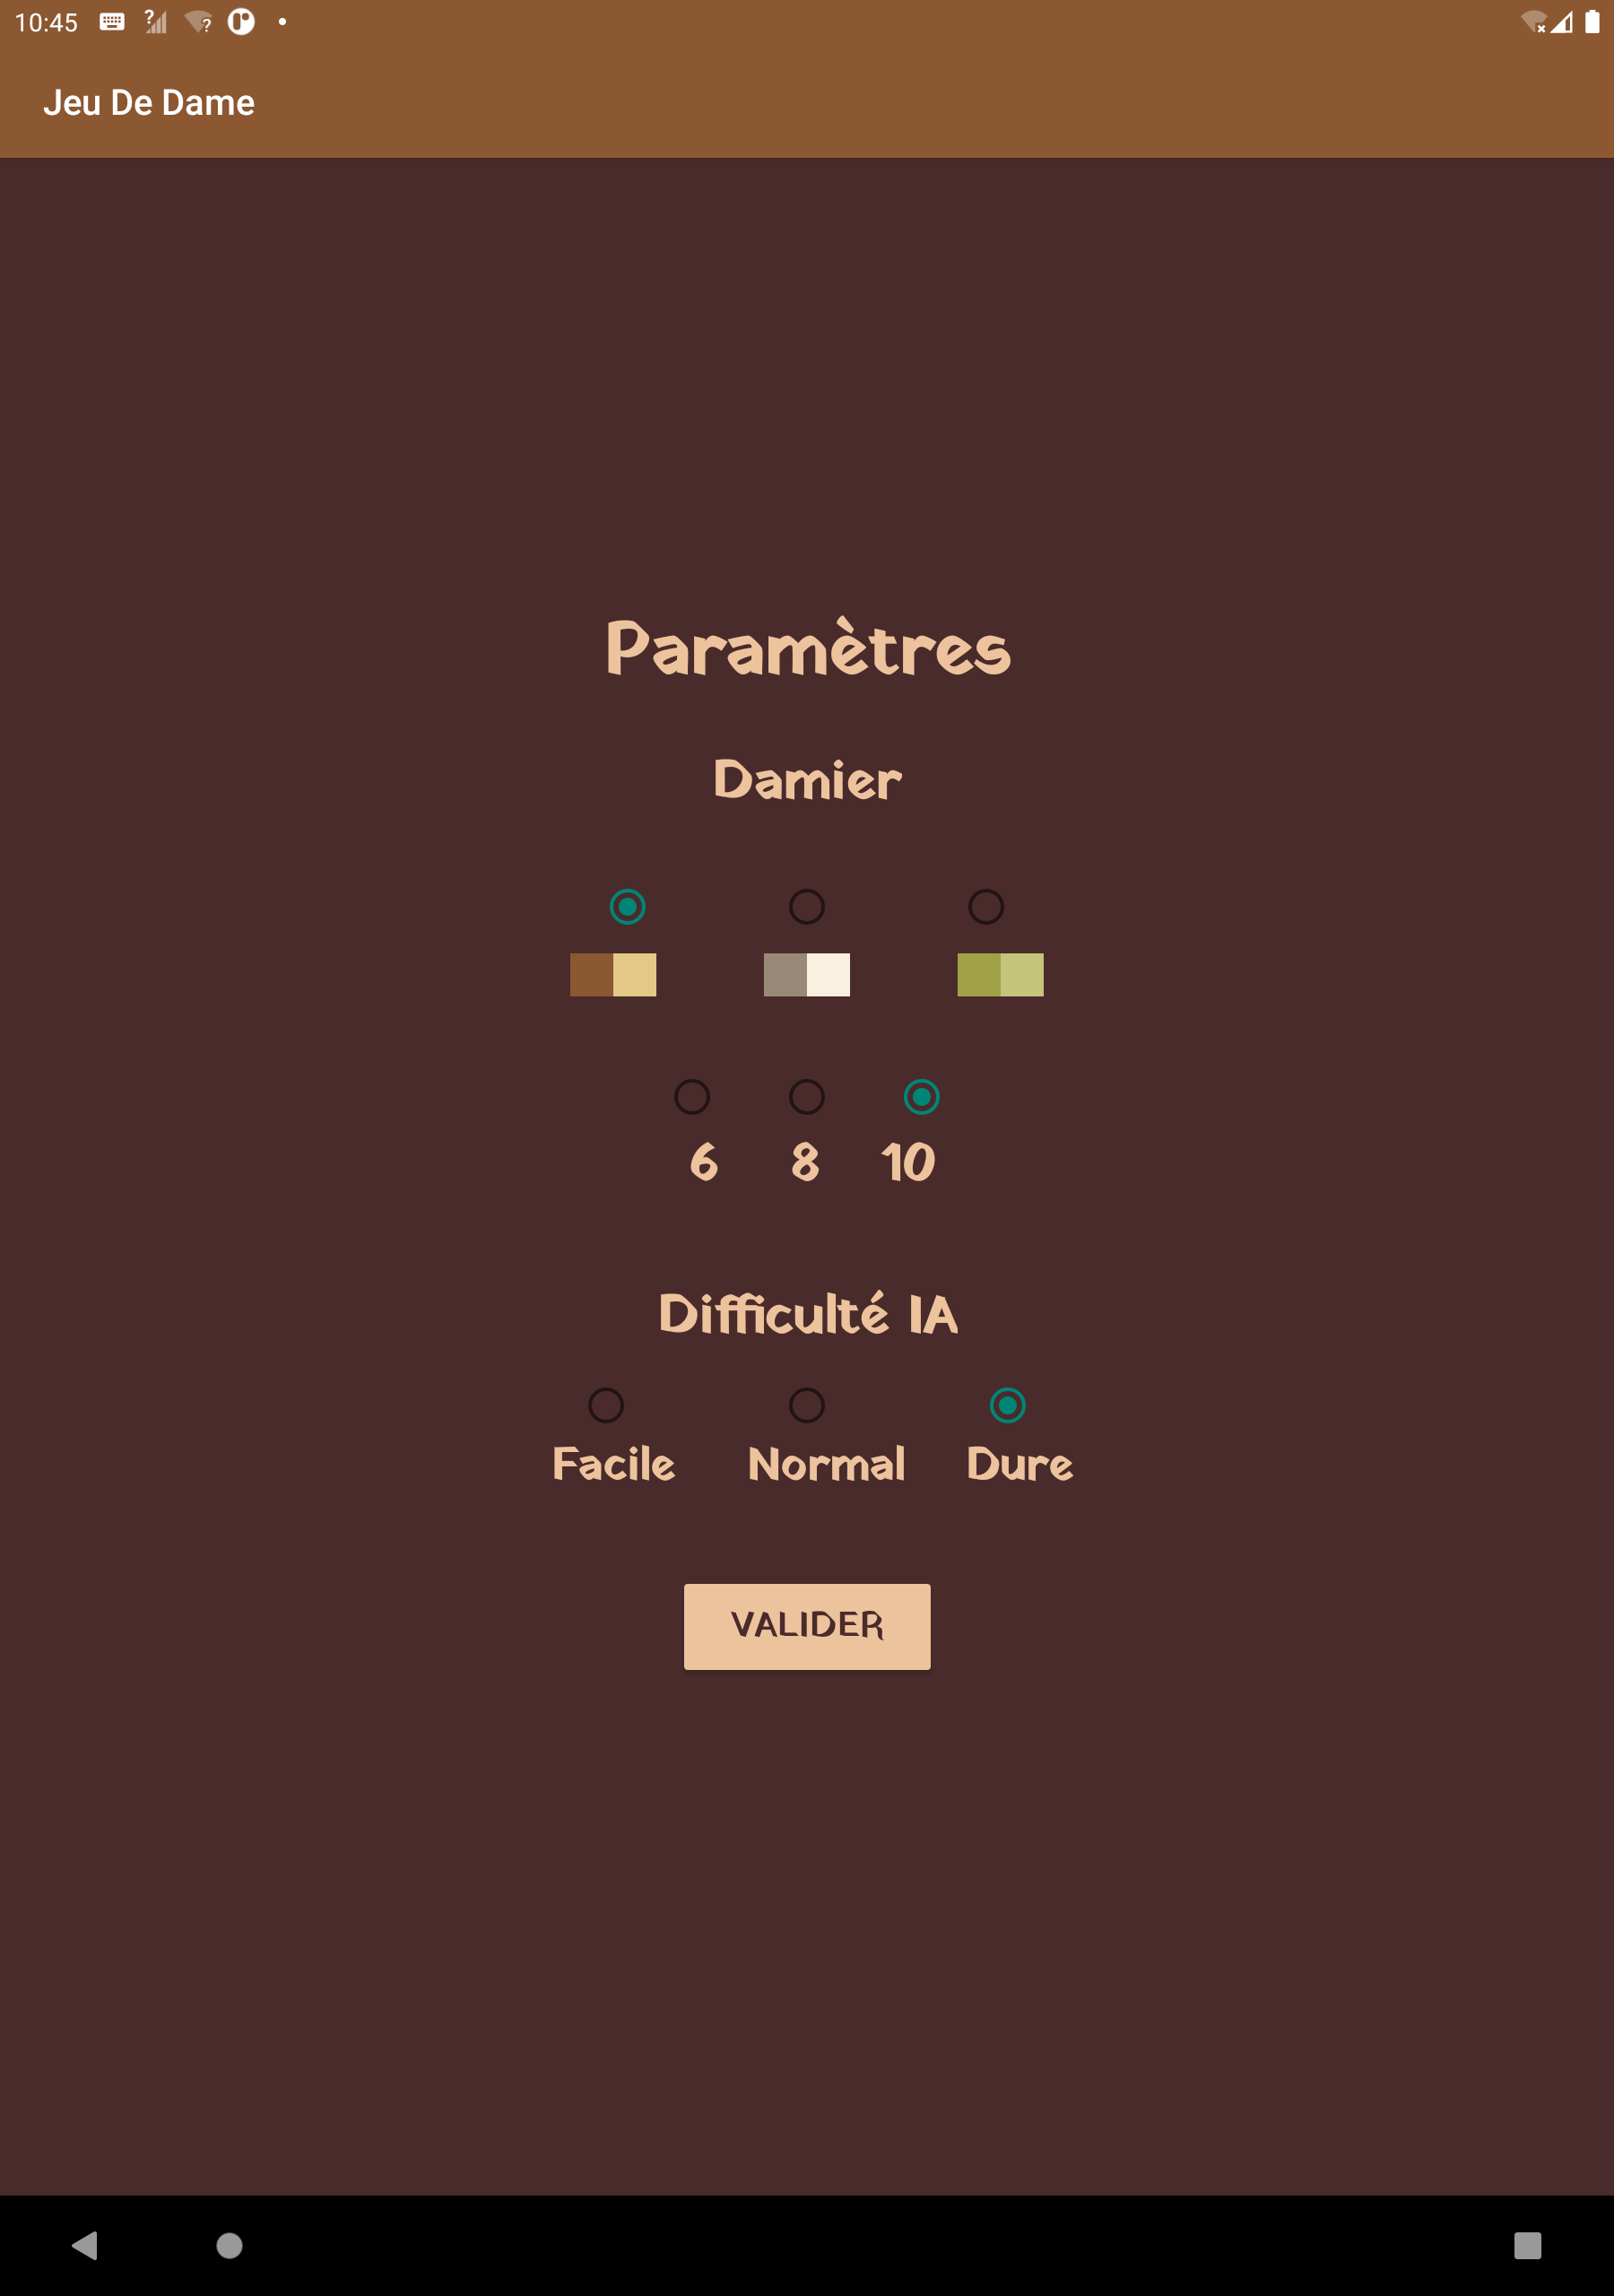
\includegraphics[scale=0.1]{setting_tablet_fr.png}
  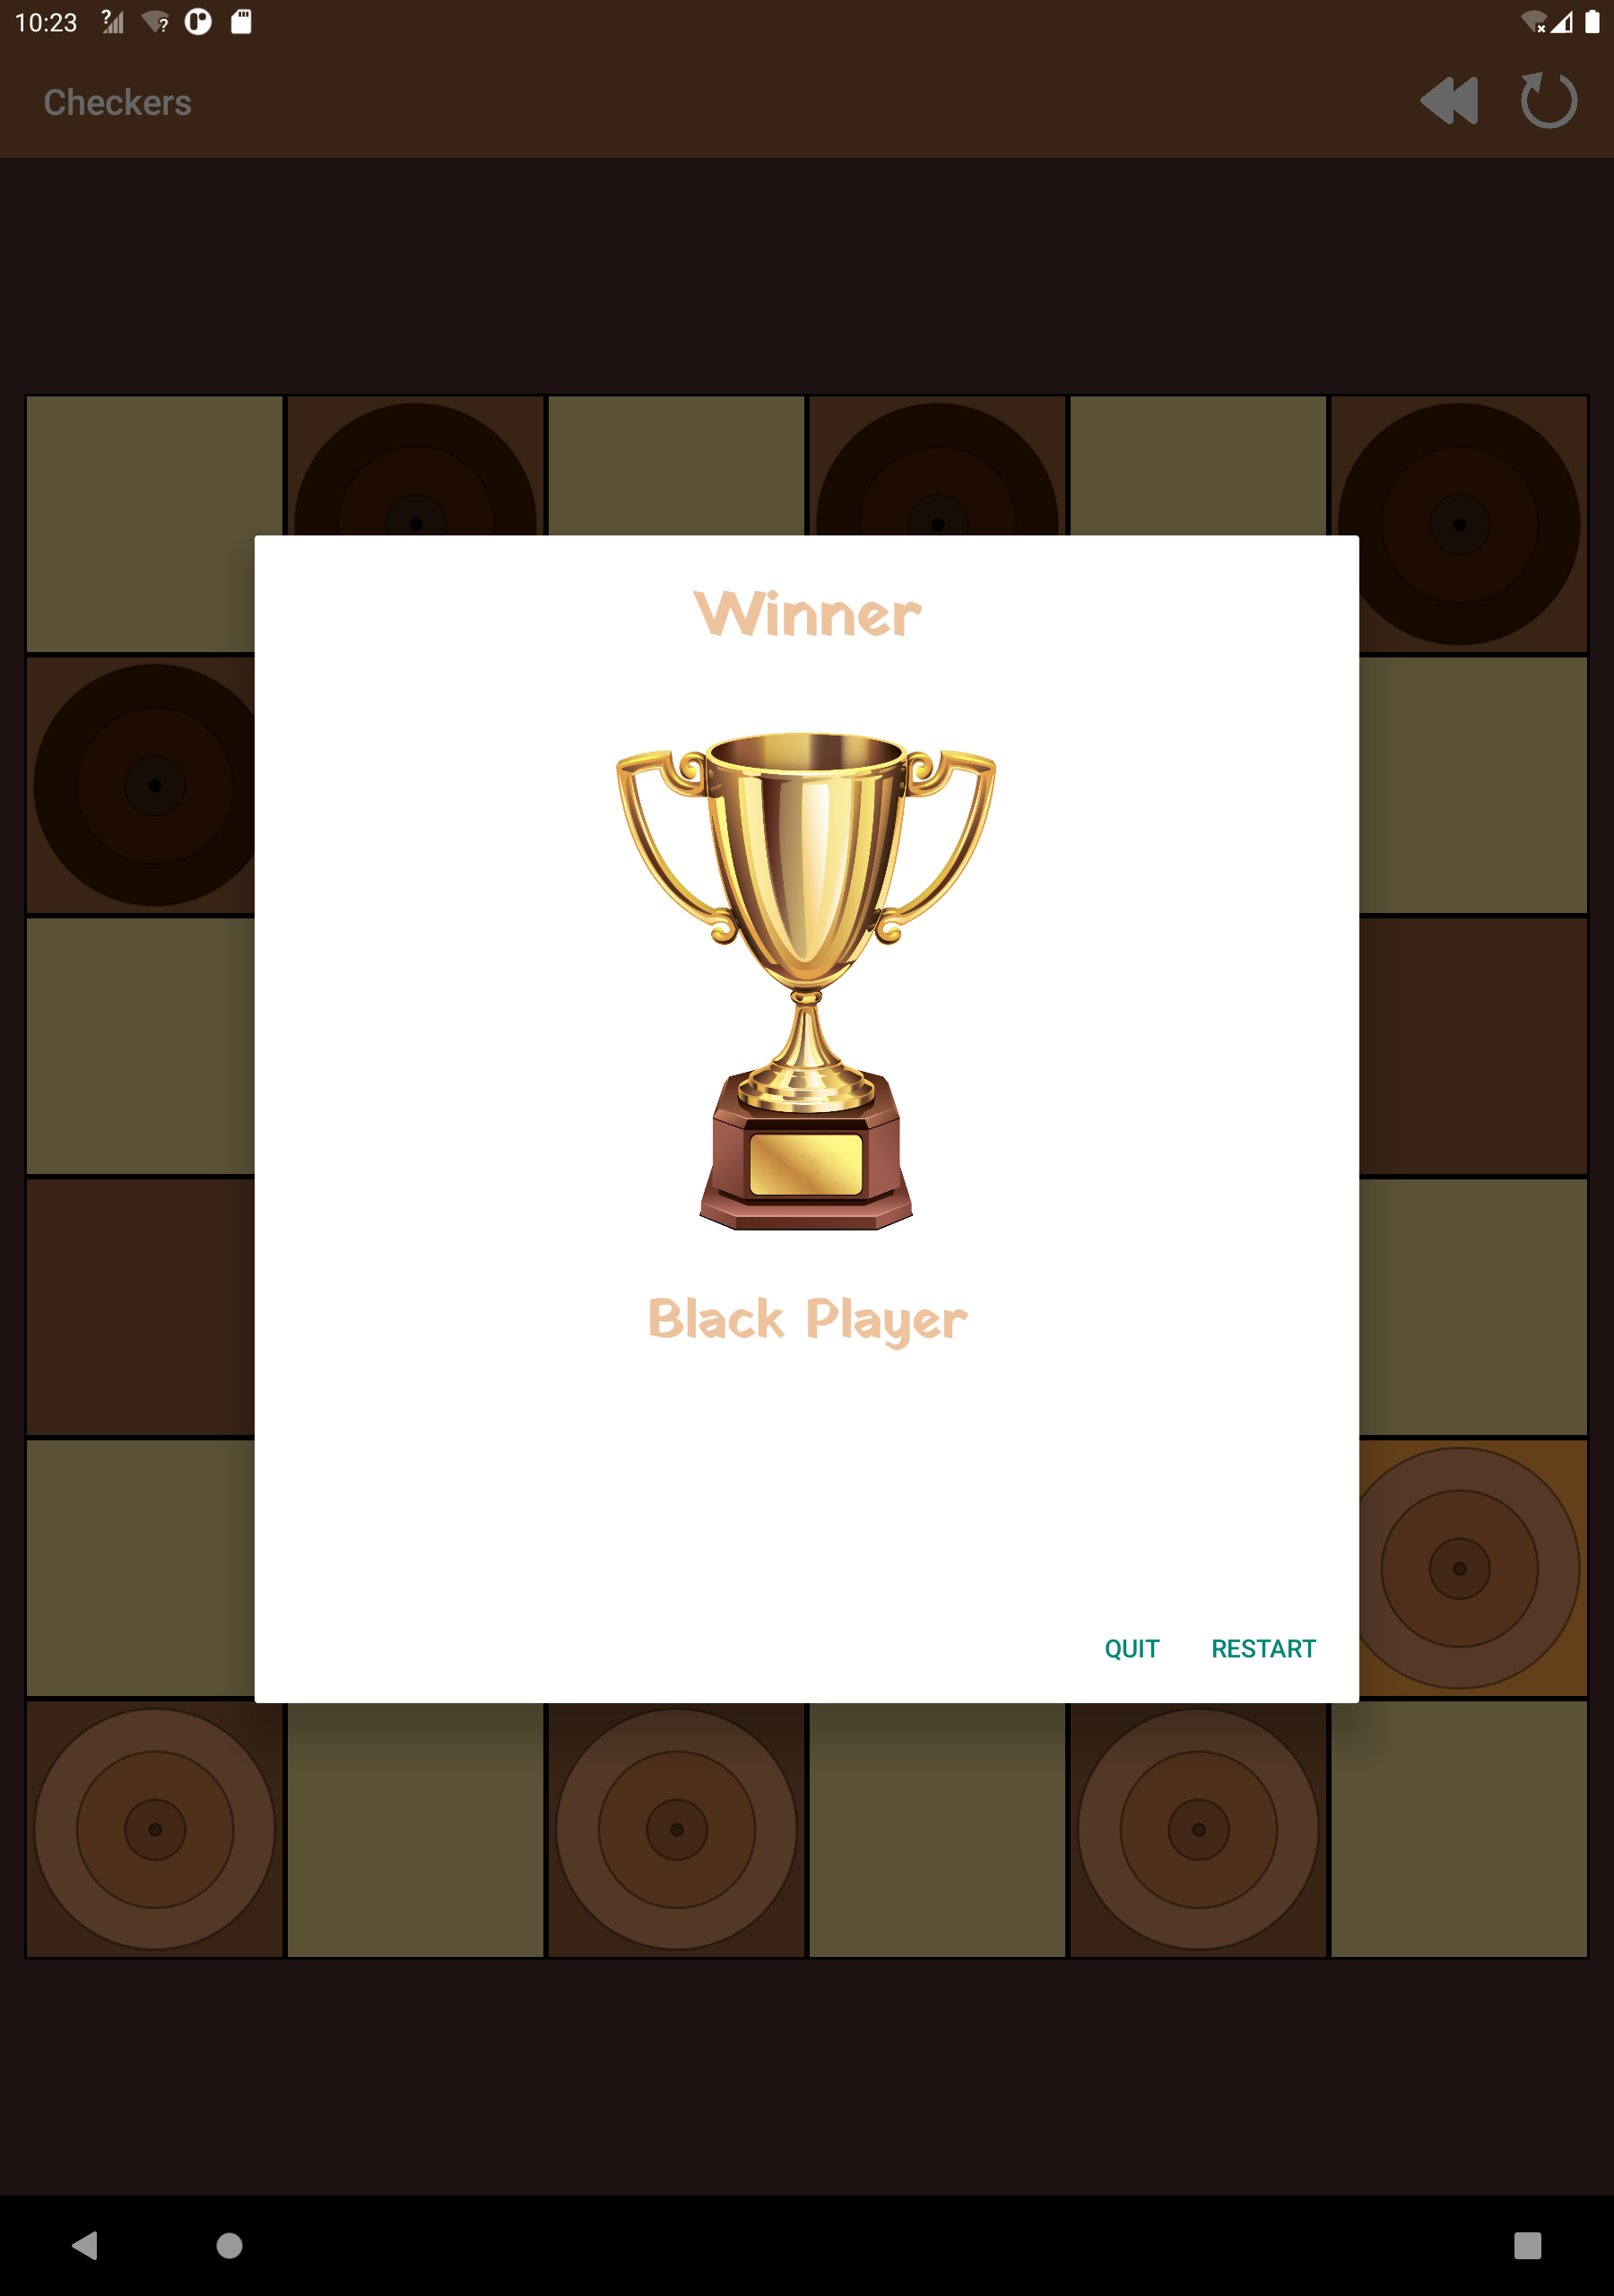
\includegraphics[scale=0.1]{pop_up_victoire_tablet.png}
\end{center}


Et enfin, un petit pop up sympa lorsqu'un joueur gagne la partie.

\section{Architecture du code}

L'implémentation du jeu est différente sur les deux plateformes.

En effet, au début du projet, nous étions parti sur une même base.

Mais pour implémenter l'IA sur Android, on a du retravailler toute la structure du code
 (ce qui fut une bonne initiative d'ailleurs)

\subsection{Android} %% une sous-section

La structure du code adoptée pour l'application sur Android se veut plus précise, plus concise et plus efficace 
mais moins académique. 

En effet, dans l'implémentation, on a évité de mettre beaucoup de classes utilitaires inutiles
comme Joueur, Plateau, Pièce, etc... 

\textbf{Voici le diagramme de classe de la version Android: }

\begin{center}
  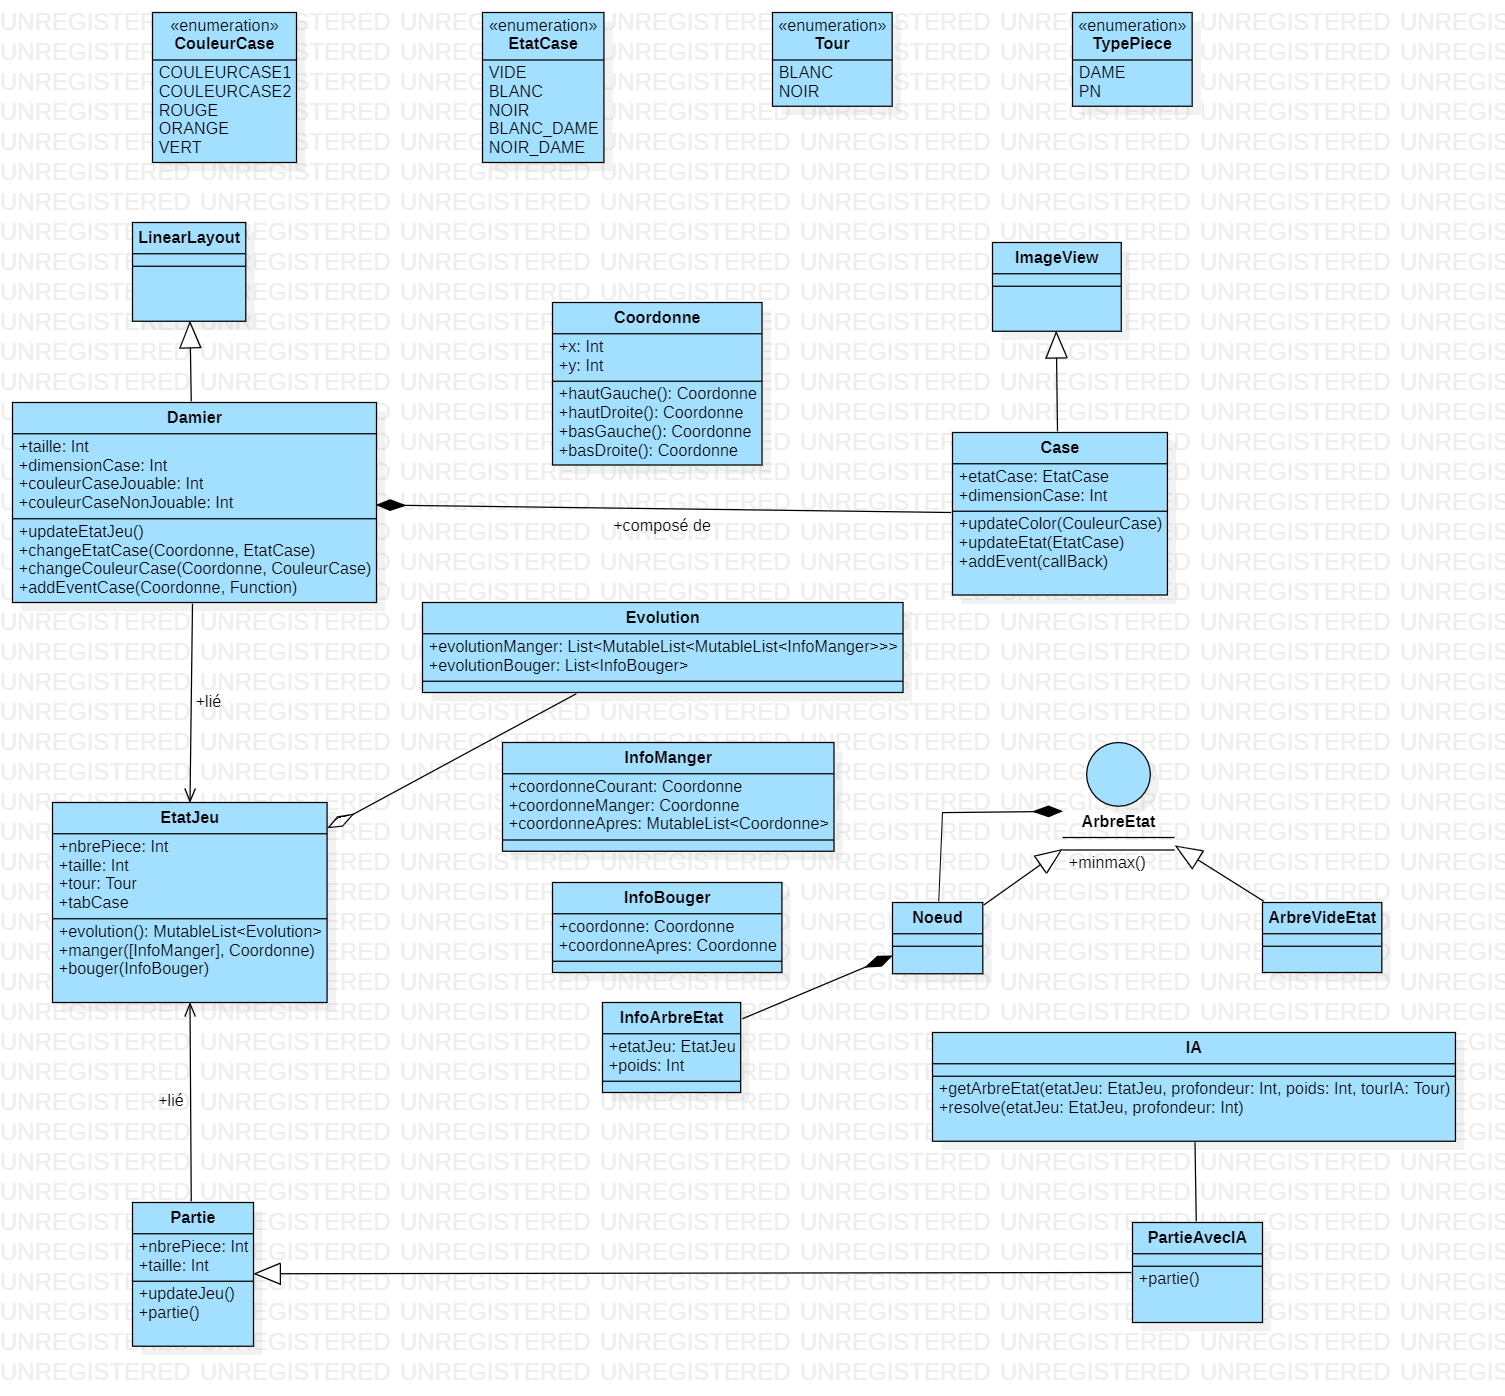
\includegraphics[scale=0.26]{diagramme_android.png}
\end{center}

En résumé:

  \subsubsection{EtatCase (Model)}

  Cette classe représente l'état du Jeu à un instant donné. 
  Cela se représente très facilement par un \textbf{List<List<EtatCase>>}

  Avec cette classe, on a la possibilité de retourner tous les évolutions possible du jeu.
  C'est-à-dire, les cases que l'on pourra manger et les endroits où on pourra se déplacer.

  Les méthodes manger() et bouger() permettent à partir des classes 
  \textbf{InfoManger} et \textbf{InfoBouger} de retourner une nouvelle \textbf{EtatJeu} avec les 
  changements adéquats.

  Cela nous permet de faire évoluer notre partie et de mettre en place un IA
  
  \subsubsection{Damier (Vue)}
  
  Cette classe est un \textbf{LinearLayout} qui va contenir des \textbf{Case} 
  qui sont des \textbf{ImageView}.

  C'est elle qui va afficher le damier et qui va mettre en place tous la partie Vue 
  de notre jeu. 
  C'est elle aussi qui gère les evenements sur les cases.

  \subsubsection{Partie (Controlleur)}
  
  Cette classe permet la liaison entre la vue \textbf{Damier} et le model \textbf{EtatCase}
  et permet de mettre en place les évènements, colorier les cases, etc... 

  En gros, elle fait fonctionner le Jeu

  \subsubsection{Setting}

  Cette classe permet la persistance des données sur les paramètres de notre jeu dans un fichier

  \textbf{Code d'implémentation : }

  \begin{verbatim}
    
    data class Setting(
    
        var colorCase: Int,
        var tailleDamier: Int,
        var profondeur: Int,
        var nbrePiece: Int = when (tailleDamier) {
            6 -> 6
            8 -> 12
            10 -> 20
            else -> 12
        }
    
    ) : Parcelable, Serializable {
    
        constructor(parcel: Parcel) : this(
            parcel.readInt(),
            parcel.readInt(),
            parcel.readInt(),
        ) {
        }
    
        override fun writeToParcel(parcel: Parcel, flags: Int) {
            parcel.writeInt(colorCase)
            parcel.writeInt(tailleDamier)
            parcel.writeInt(profondeur)
        }
    
        override fun describeContents(): Int {
            return 0
        }
    
        companion object CREATOR : Parcelable.Creator<Setting> {
            private val seralVersionUid: Long = 12323465
            override fun createFromParcel(parcel: Parcel): Setting {
                return Setting(parcel)
            }
    
            override fun newArray(size: Int): Array<Setting?> {
                return arrayOfNulls(size)
            }
        }
    }

    fun persisteSetting(context: Context, setting: Setting) {
        val fileOutput = context.openFileOutput("setting.txt", Context.MODE_PRIVATE)
        val outputStream = ObjectOutputStream(fileOutput)
        outputStream.writeObject(setting)
        outputStream.close()
    }

    fun loadSetting(context: Context): Setting {
        val fileInput = context.openFileInput("setting.txt")
        val inputStream = ObjectInputStream(fileInput)
        val setting = inputStream.readObject() as Setting
        inputStream.close()
        return setting
    }
    

  \end{verbatim}

  \subsubsection{IA}

  Cette classe est une implémentation d'une classe anonyme (Une bibliothèque)

  Elle contient la fonction resolve() qui à partir d'un \textbf{EtatJeu} 
  de deduire le meilleur coup possible.

\subsubsection{Extrait de code de la fonction minMax}

\begin{verbatim}
  fun minMax(tourIA: Tour): Int {

        return when(this) {

            is ArbreVideEtat -> 0
            is NoeudArbreEtat ->

                if ( fils.all { it is ArbreVideEtat } ) infoArbreEtat.poids
                else {

                    if (infoArbreEtat.etatJeu.tour === tourIA) 
                        max(fils.map { it.minMax(tourIA) } as MutableList<Int>)
                    else min(fils.map { it.minMax(tourIA) } as MutableList<Int>)

                }
            else -> 0
        }

    }

\end{verbatim}

\subsubsection{Extrait de code de génération de l'arbre des possibles}

La fonction d'évaluation utilisé 

\begin{verbatim}

  fun getArbreEtat(
    etatJeu: EtatJeu,
    profondeur: Int,
    poids: Int = 0,
    tourIa: Tour = etatJeu.tour
  ): ArbreEtat {

      return when {
          profondeur === 0 -> ArbreVideEtat
          etatJeu.evolution().isEmpty() -> NoeudArbreEtat(
              infoArbreEtat = InfoArbreEtat(etatJeu, poids), 
              fils = mutableListOf(ArbreVideEtat)
          )
          else -> NoeudArbreEtat(
              infoArbreEtat = InfoArbreEtat(etatJeu, poids),
              fils = etatJeu.evolution().map {
                  getArbreEtat(
                      it.etatJeu,
                      profondeur - 1,
                      poids + 
                      if (tourIa === it.etatJeu.tour) 
                        -1 * it.poids 
                      else it.poids
                  )
              } as MutableList<ArbreEtat>
          )
      }

}

\end{verbatim}


\subsection{iOS} %% une autre sous-section

\begin{center}
  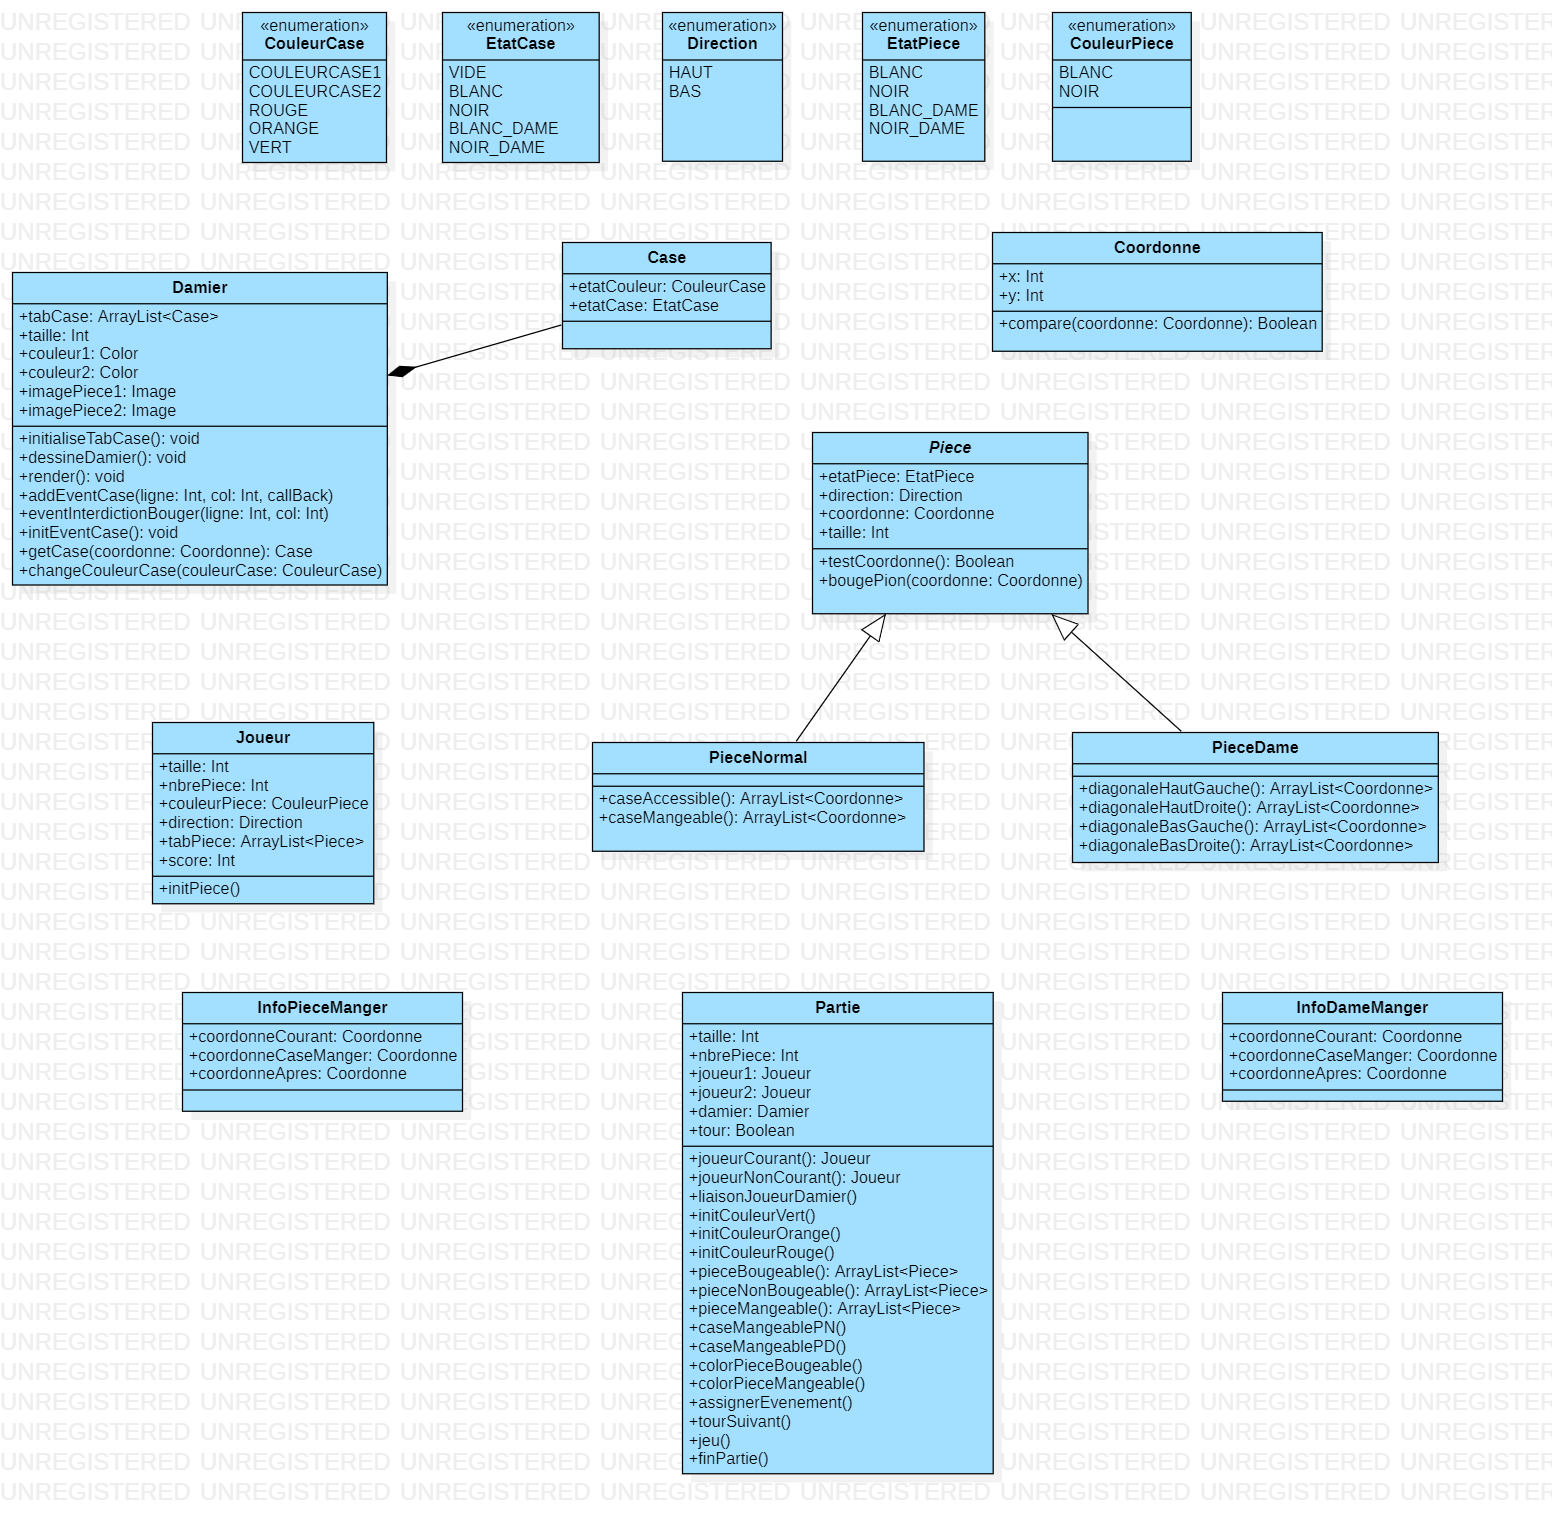
\includegraphics[scale=0.26]{diagramme_iospng.png}
\end{center}

Cela fonctionne comme précedemment mais sans IA


\section{Quelques points délicats/intéressants}

\subsection{Points Intéressants}

\begin{itemize}
  \item On a utilisé à plusieurs reprises de la réccursivité dans le code.
  \item Le critère d'évaluation utilisée pour l'algorithme MiniMax est le nombre de pièce manger.
  \item La profondeur de l'arbre utilisé pour l'algorithme minimax varie entre 2 (facile) à 4 (difficile).
  \item On peut monter au maximum jusqu'à huti pour la profondeur de l'arbre pour minMax.
  \item L'IA avec une profondeur de trois est déjà très durs à battre.
  \item Je vous recommande, d'aller voir le code sur GitHub, 
  on a éssayer de faire un code propre et très facilement lisible.
\end{itemize}

\subsection{Point délicat}

\begin{itemize}
  \item Les règles de jeu de dame est assez durs à implémenter. On a du 
  changer plusieurs fois la manière de les implémenter pour que celà fonctonne parfaitement.

  Cependant, je suis convaincu que cela à améliorer nos compétences en génie logiciel.

  \item L'implémentation de l'IA n'était pas évident.
  
  \item Aucune implémentation de liste a été faite par manque de temps
  
\end{itemize}

\section{Conclusion}

 Pour conclure, ce projet était très enrichissant d'une part le 
 fait que ce soit sur Mobile et d'autre part, qu'on a dû se surpasser pour le réussir.

 On est satisfait de ce qu'on a pu accomplir, surtout sur Android, où on a pu implémenter une IA.

%%% La bibliographie:
\bibliographystyle{plain}
\bibliography{ma_biblio}

\end{document}
